% corresponds to IESA 2017-04-10


% 2019-03-27

\documentclass[10pt]{article}
\usepackage[T1]{fontenc}
\usepackage{amssymb}
\usepackage{amsmath}
\usepackage{graphicx}
% \begin{figure}[h]
% \centering
% \includegraphics[width=6.5in]{folder/photo.png}
% \caption{}
% \label{}
% \end{figure}



\usepackage{tikz}
\usetikzlibrary{arrows}
\usepackage{subfigure}
\usepackage{stackrel}
\usepackage{blindtext}

\usepackage{biblatex}
\addbibresource{library.bib}

\oddsidemargin=0.15in
\evensidemargin=0.15in
\topmargin=-.5in
\textheight=9in
\textwidth=6.25in

\usepackage[colorlinks=true,breaklinks,pdfpagemode=none,linkcolor=blue,citecolor=blue]{hyperref}

\usepackage{enumerate}
% \vspace{-6pt}
% \begin{itemize}
%     \setlength{\itemsep}{0pt}%
%     \setlength{\parskip}{0pt}%
%     \item Item 1
%     \item Item 2
%         \begin{itemize}
%             \setlength{\itemsep}{0pt}%
%             \setlength{\parskip}{0pt}%
%             \item Sublist Item 1
%             \item Sublist Item 2
%         \end{itemize}
%         \item Item 3
% \end{itemize}
% \vspace{-6pt}


\usepackage{enumitem}
\setlist{itemsep=0mm}

\usepackage{amsmath,amsfonts,amssymb,bm}


\begin{document}

   \noindent
   \begin{center}

   \hrulefill
   
   \vspace{5pt}
   
   \makebox[\textwidth]{ {\bf Energy Systems Analysis} \hfill  A.D. Smith 2019}
   \vspace{0pt}
   
   {\Large \hfill  Lecture 26.  
Global Sensitivity Analysis (GSA) for Models
}
   \vspace{5pt}
   
  
   \hrulefill
   \end{center}

 {\color{darkgray}{\center{ \small{      ``In \textit{global SA}, the aim is to apportion the uncertainty in the output variable to the uncertainty in each\\ input factor.''
\\%[3pt]
\rightline{{\rm --- Campolongo et al. in Ch. 2 of \cite{Campolongo2000-ds}}}}}}}

\section{What is global sensitivity analysis?}

Global sensitivity analysis (GSA) tells us how (or whether) a variation in one thing (a model input) causes variation in another thing (a model output), but goes beyond a local derivative-based method to try and capture the response across a wide range of system behaviors. 

\begin{description}
\item [\textbf{Global sensitivity analysis}] is  ``the study of how the uncertainty in the output of a model (numerical or otherwise) can be apportioned to different sources of uncertainty in the model input.'' \cite{Saltelli2004-ga}
\end{description}



\subsection{Compared with simple, local derivative-based sensitivity analysis}

The simplest method for obtaining a sensitivity index, as discussed in the previous lecture, is to obtain a local derivative. For modelers, this means fixing all factors except the one for which you are obtaining a sensitivity, then varying that factor of interest. This is called a one-at-a-time (OAT) or simple sensitivity analysis. Saltelli cautions: ``Differential analysis [local derivative-based SA] can be used with caution when the range of variation of the factors is small. Some methods\ldots perform poorly for nonlinear, non-additive models.'' \cite{Saltelli2009-tz}

%\medskip

A GSA goes beyond this by incorporating:

\vspace{-8}
\begin{itemize}
    \setlength{\itemsep}{0pt}%
    \setlength{\parskip}{0pt}%
    \item Scale and shape
    \item Effect(s) of stochastic variation in the input(s) on the output(s)
    \item Range of possible values or probability distributions possible for the input(s)
\end{itemize}
\vspace{-6}

If a local derivative is assumed to be representative in a model that is actually complex and nonlinear, or if uncertainty is neglected, this ``might result in an under-estimation of predictive uncertainty and an incomplete understanding of the input-output relationship.'' \cite{Saltelli2004-ga}

\subsection{Paired with uncertainty analysis}

Saltelli cautions: ``Local methods are less helpful when SA is used to compare the effect of various factors on the output, as in this case the relative uncertainty of each input should be weighted.'' \cite{Saltelli2009-tz}


\section{Capturing more complexities}


Let's briefly describe a few key terms that will be used in our discussions. 

\vspace{-6}
\begin{description}
\item [\textbf{Sensitivity   index}] A   derivative-based   valuation   of   how   influential   a   factor,   or   input   variable,   is   on
an   output   of   interest. \cite{Saltelli2004-ga}
\item [\textbf{Main effect}] A `first order effect'  that is based on the variance of the output of interest with the factor fixed at its  (estimated) midpoint; i.e. ``If we could eliminate   the  uncertainty in one of the [inputs], making   it into a constant, how much would this reduce  variance of [the output]?'' \cite{Saltelli2004-ga}
\item [\textbf{Total effect}] A   higher-order   effect   that   is   based   on   the   variance   of   the   output   of   interest over   all   possible   values   of   the   factor---an   attempt   to   capture   the   total    contribution   to   the variation   in   model   output   due   to   this   factor.
\end{description}



For the energy modeler, it may well be the case that ``factors in a model follow a very asymmetric distribution of importance, few factors accounting for most of the output uncertainty with most factors playing little or no role.'' \cite{Saltelli2004-ga}

\subsection{Interactions (Complex and nonlinear models)}

    The sensitivity index gives us a metric for understanding the response of one variable (output) to another (input), as described in the previous lecture. When we refer to 'sensitivity index' without additional context, this is taken to mean a first-order effect.

The first-order effect is a number, scaled between 0 and 1, representing the sensitivity to a certain factor. If the input factors are independent (non-interacting), the sum of the first order effects (when normalized) should be 1. Unity represents the combined sensitivity to all features. Therefore, in that case we can think of the first order effect as being a fraction representing that particular factor's influence on the outcome.

If the input factors are not independent, the sum of the first order effects (when normalized) will \textit{not} be 1. If the combination of the first-order sensitivity indices never reaches 1, that indicates we haven't completely captured the full picture of the influences of the relevant factors throughout the process. This could be an indication that we have interactions between the factors. The effect of an interaction between two factors can also be called a two-way or second-order effect.

The total effect is ``the sum of all the sensitivity indices involving the factor in question.'' \cite{Saltelli2009-tz} It is a number that has been normalized in the same way as the first-order effect, but the total effects will not sum to 1. In fact, for the case of interacting factors where the first-order effects sum to less than 1, the total effects will be greater than 1. This is because the total effect captures sensitivity behaviors in the model related to variance in the factor and due to all interactions involving that particular factor of interest. The total effect can also be called a total sensitivity index \cite{Saltelli2009-tz}.

For any individual factor, looking at its main effect and total effect estimates together can be informative or even illuminating. Without these calculations, the linear effects may be evident from the first-order indices, while the nonlinear effects may not be evident.


\section{Do I need GSA methods?}

Your time and computational resources may limit your choices on how much analysis you can do, but here are a few questions to ask that would indicate you should look further into GSA methods:

\vspace{-6}
\begin{itemize}
    \setlength{\itemsep}{0pt}%
    \setlength{\parskip}{0pt}%
    \item Is the model nonlinear? Do you know or suspect that the factors are interacting with each other?
    \item Are your input factors ``affected by uncertainties of different orders of magnitude?'' \cite{Saltelli2009-tz}
    \item Have you performed a simple (local derivative or parametric) sensitivity analysis and found that the results are not as useful as you expected, or that they don't make sense based on your understanding of the system?
\end{itemize}
\vspace{-6}

An in-depth sensitivity analysis of a system model can help us to find ``where [we] should improve our knowledge in order to reduce the risk of failure.'' \cite{Saltelli2004-ga} This may drive model improvements and improved or additional data collection procedures as well as improving understanding of the model's behavior. Interestingly, a thorough SA may also help us to decide what model to use or how a system ought to be modeled: ``Sensitivity analysis can be employed also when dealing with uncertain or competing model structures or scenarios, treating the choice of the model as one of the sources of uncertainty.'' \cite{Saltelli2000-jo}


\section{Desirable properties for GSA}

Some of the most important benefits of a high-quality sensitivity analysis are summarized in this list adapted from Saltelli \cite{Saltelli2009-tz}:

\begin{enumerate}
    \setlength{\itemsep}{0pt}%
    \setlength{\parskip}{0pt}%
    \item Ability to cope with influence of scale \& shape
    \item Evaluation of a factor's effects while all other factors are also varying
    \item \textbf{Efficiency:} Accounting for the challenges above in a way that is manageable computationally.
    \item \textbf{Model Independence:} Works with models that are not necessarily additive or linear
    \item \textbf{Simplicity:} Independent of factor grouping (to help interpretability of the results, in additional to increasing efficiency)
\end{enumerate}

\section{Global properties for GSA}

\begin{enumerate}
    \setlength{\itemsep}{0pt}%
    \setlength{\parskip}{0pt}%
     \item ``\textbf{The inclusion of scale and shape}: The sensitivity estimates of individual factors incorporate the effect of the range and the shape of their probability density functions.'' \cite{Saltelli2009-tz}
     \item ``\textbf{Multidimensional averaging:} The sensitivity estimates of individual factors are evaluated varying all other factors as well.'' \cite{Saltelli2009-tz}

\end{enumerate}

This is the most concise summary I have seen describing the benefits of, and the need for, GSA.

\section{How to perform a (global) sensitivity analysis}

The steps shown in the previous SA lecture (adapted from \cite{Saltelli2009-tz}) were actually entirely applicable to a more detailed SA, and are reproduced here.

\begin{enumerate}
    \setlength{\itemsep}{0pt}%
    \setlength{\parskip}{0pt}%
    \item Design the modeling experiment (identify what question the model should answer) and determine which of the input factors you are concerned with in the analysis.
    \item Assign a range of variation to each input factor (and a probability density function, if you have a known or estimated distribution).
    \item Evaluate the model, creating an output distribution for the response(s) of interest.
    \item Assess the influence or relative importance of each input factor you are concerned with on the output variable(s).
\end{enumerate}

% \noindent{}
% GSA methods may be further divided into \cite{Saltelli2009-tz}:
% \begin{enumerate}
%     \setlength{\itemsep}{0pt}%
%     \setlength{\parskip}{0pt}%
%     \item Sampling-based methods that use randomized sampling methods, also called Monte Carlo analysis
%     \item Variance-based methods that emphasize including the measured or estimated variance in the input factor(s)
%     \item Reliability methods that emphasize investigations related to  particular failure mode(s) that is/are of concern
%     \item Bayesian statistical methods that use Bayesian inference and emphasize decision making based on feasibility and desired outcome(s)
%     \item Graphical methods that provide visualizations to assist the modeler in analyzing multidimensional data
% \end{enumerate}

% These methods may be used in combination with each other, and other methods exist for other goals, depending on the modeler's needs.

Saltelli \cite{Saltelli2009-tz} also provides a diagram that illustrates this procedure, including sampling-based analysis and output distribution, as shown in Figure \ref{flowchart}.

%\medskip
            \begin{figure}[h]
            \centering
            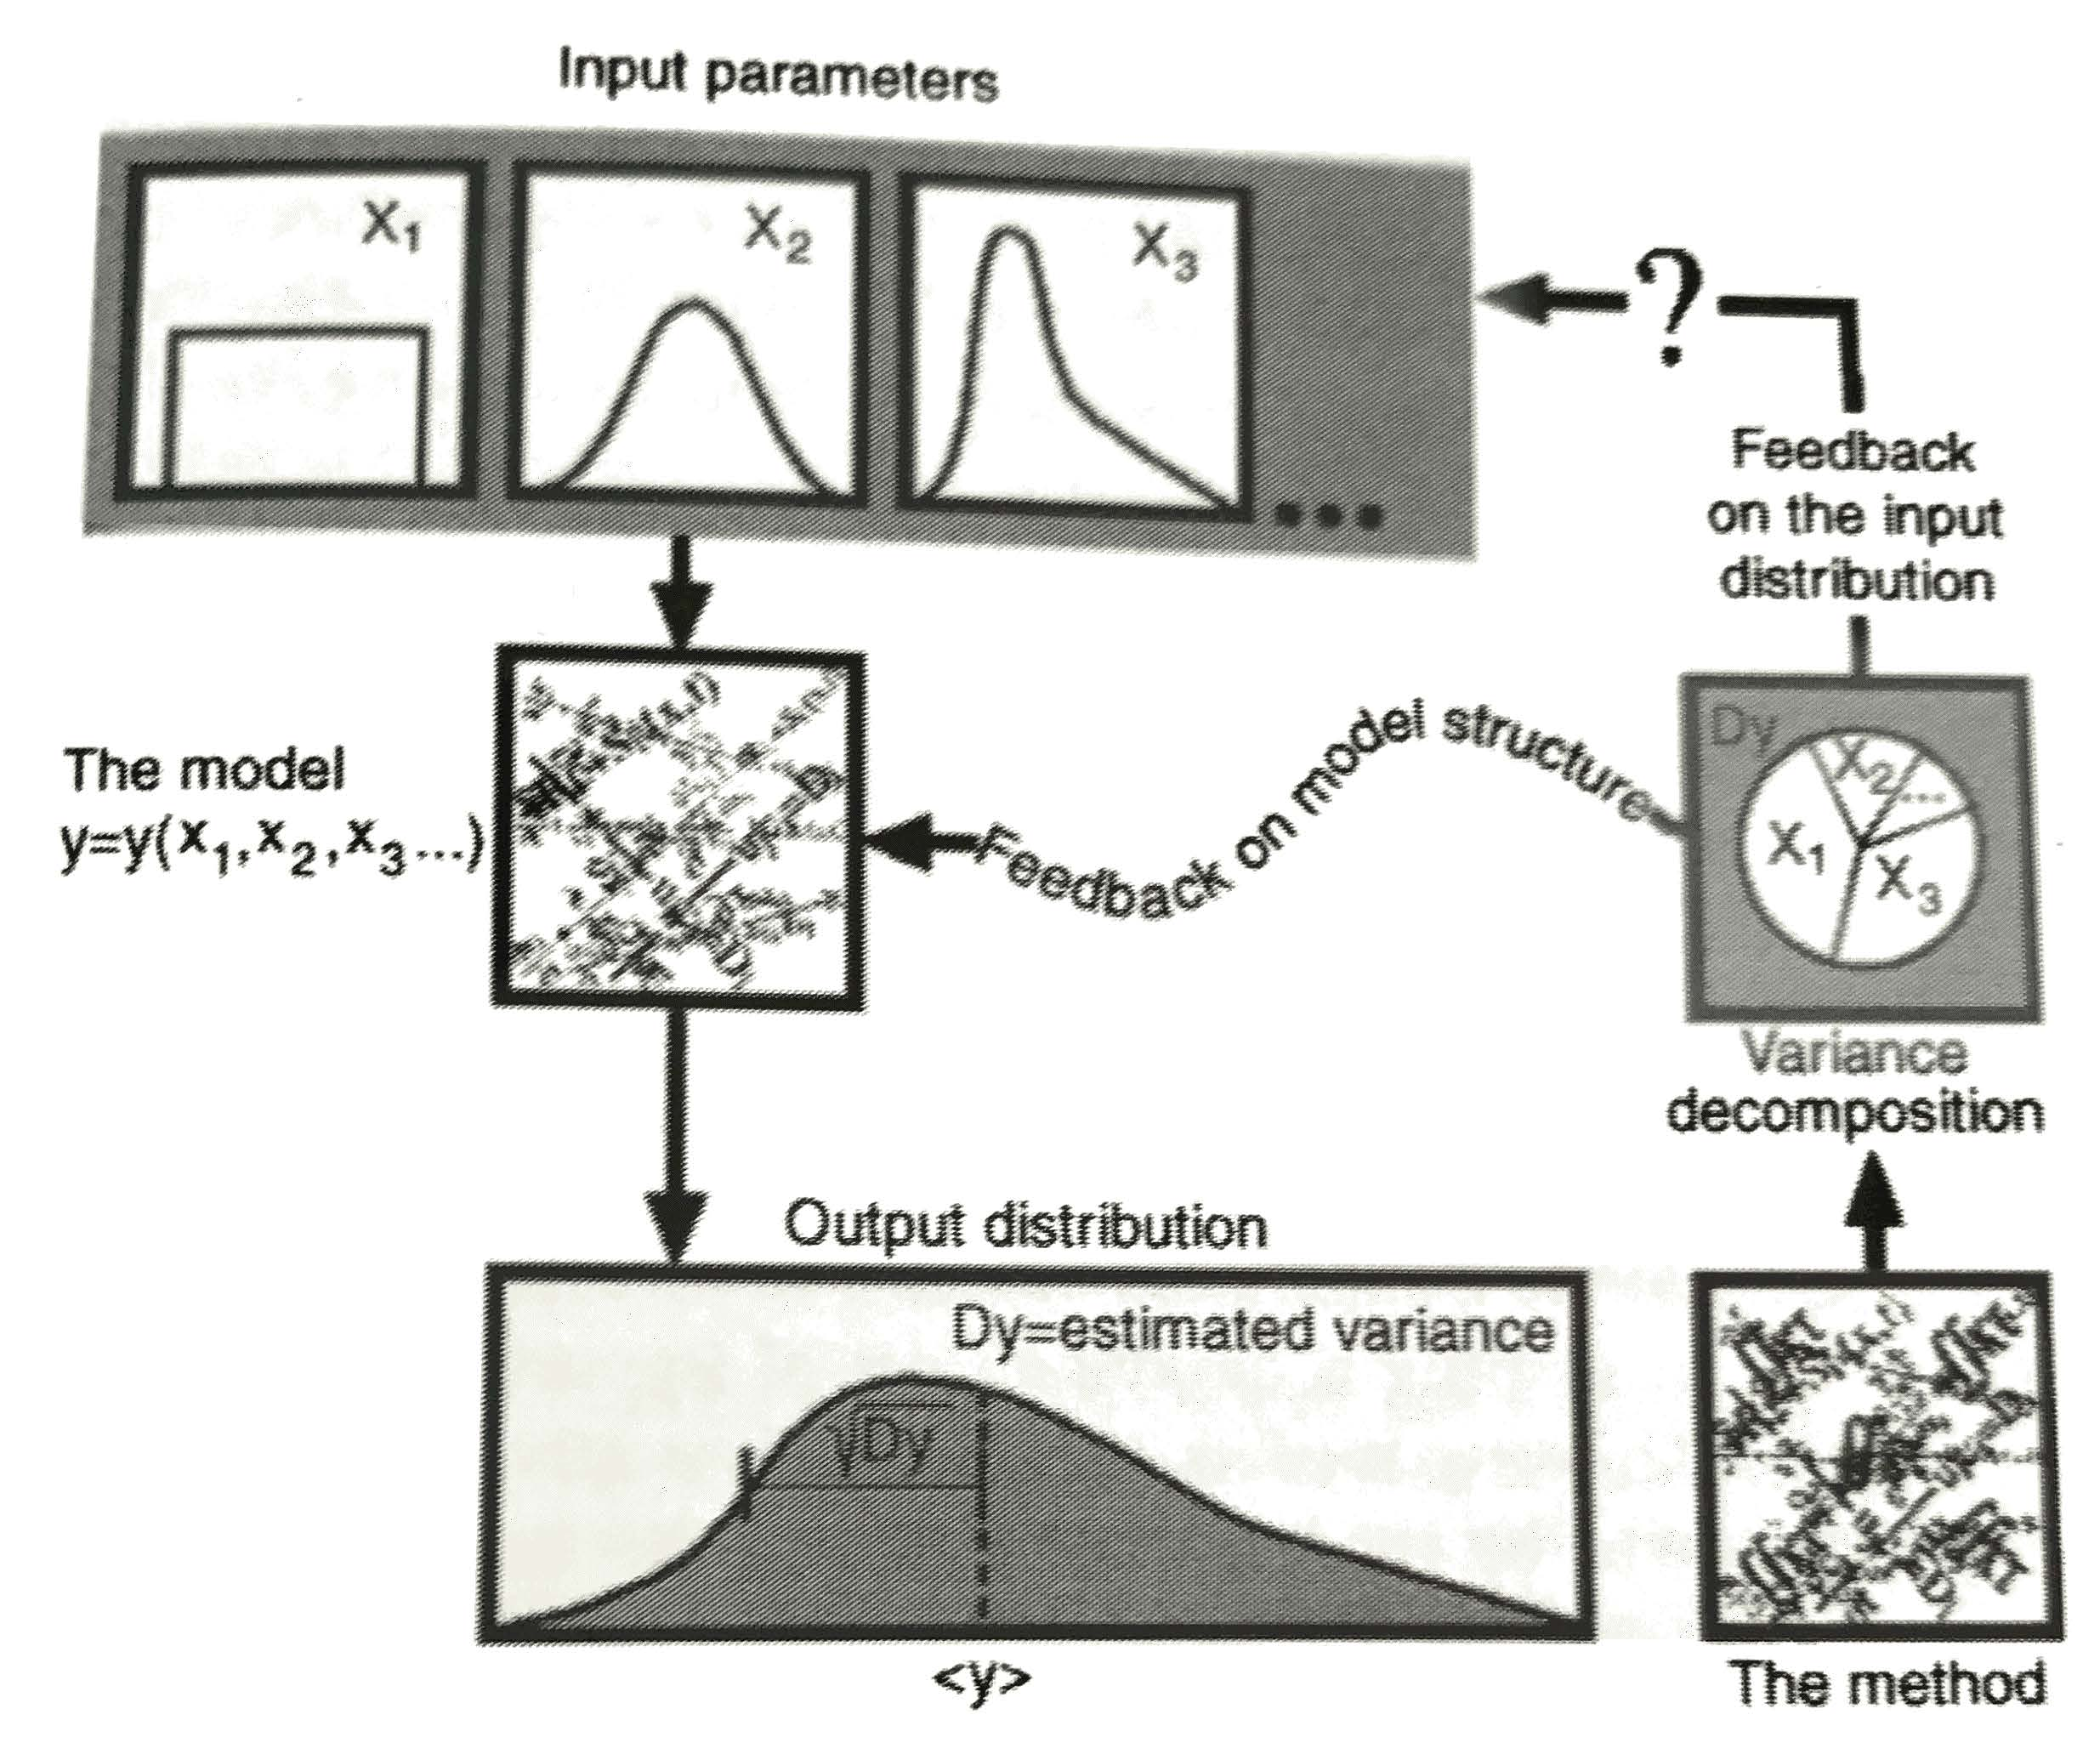
\includegraphics[width=9cm]{extras26/flowchart}
            \caption{Schematic view of sampling-based sensitivity analysis \cite{Saltelli2009-tz}}
            \label{flowchart}
            \end{figure}
%\bigskip


\section{Probability Distribution Functions (PDF)}

As illustrated in Fig. \ref{flowchart}, knowledge of the distribution (or likely distribution) of the input(s) is beneficial for the modeler using SA, as it can allow him or her to provide an expected distribution for the output(s). One key thing to understand is that ``for continuous probability distributions, PROBABILITY = AREA.'' \cite{Illowsky2014-stats}

% If you haven't had any probability or statistics, it's time to improve your understanding. Here are two free textbooks to check out from the OpenStax project:\\

% \href{https://cnx.org/contents/MBiUQmmY@18.54:kcV4GRqc@9/}{Introductory Statistics} \cite{Illowsky2014-stats}\\ 

% \href{https://cnx.org/contents/HLT_qvJK@6.2:wsOQ6HtH@8/}{Applied Probability} \cite{Pfeiffer2009-prob}\\




\subsection{Uniform distribution}

A uniform distribution means there is an equal likelihood of any value along a specified range. When you do a typical parametric analysis, or when you perform sensitivity analysis without using probability densities, you are usually implicitly assuming a uniform distribution.

%\medskip
            % \begin{figure}[h]
            % \centering
            % 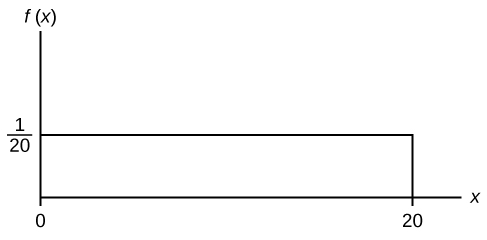
\includegraphics[width=6cm]{extras26/uniform}
            % \caption{Uniform distribution \cite{Illowsky2014-stats}}
            % \label{uniform}
            % \end{figure}
%\bigskip

\subsection{Gaussian or normal distribution}  \label{stats}

The Gaussian, or normal, distribution is frequently encountered in experiments and frequently used by modelers. It is identified by two key items: the mean, or center of the distribution, and the variance or standard deviation, both of which describe the ``spread'' of the data. Remember that the standard deviation is simply the square root of the variance.


% \begin{labeling}{Standard deviation x}
% \item [\textbf{Mean}] Average calculated by summing all values in the sample and dividing by the number of values in the sample. Typically symbolized by $\mu$.
% \item [\textbf{Standard deviation}] An indicator of how far away from the mean the data will be. Moving one standard deviation in both directions from the center of a normal distribution will capture just over 2/3 of the data points. Typically symbolized by $\sigma$.
% \item [\textbf{Variance}] A descriptor of the variance in the data, calculated as follows. Typically symbolized by $\sigma^2$.
% $$ \sigma^2 = \frac{1}{n-1} \sum{(x-\mu)^2} $$
% where $n$ is the number of data points in the sample, $x$ is an individual data point, and the summation is made over all $x$ values (from 1 to n).
% \end{labeling}


%\medskip
            % \begin{figure}[h]
            % \centering
            % 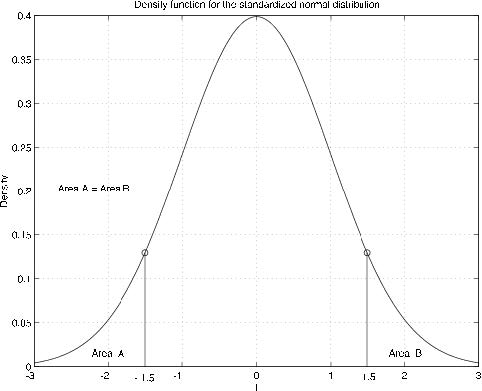
\includegraphics[width=8.5cm]{extras26/Gaussian}
            % \caption{Standardized normal distribution \cite{Pfeiffer2009-prob}}
            % \label{reflabel}
            % \end{figure}
%\bigskip

The distribution is often normalized (to allow for the use of lookup tables, and comparisons across disparate applications) so that its total area is 1. If you want to find the probability of landing below or above a certain value, or landing between two values, in a normal distribution, you just integrate. Fig. \ref{int} illustrates a more complex distribution where the analyst wants to find the probability of landing in between values $a$ and $b$.

%\medskip
            \begin{figure}[h]
            \centering
            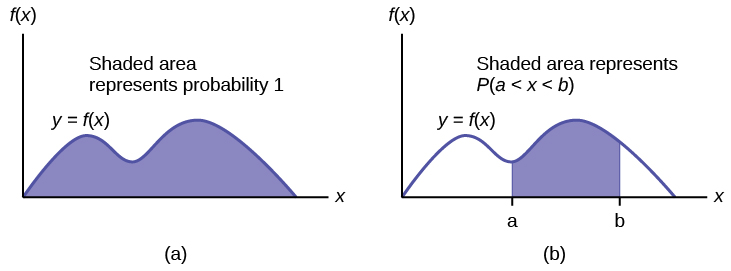
\includegraphics[width=11.5cm]{extras26/PDFintegration}
            \caption{Integrating a PDF \cite{Illowsky2014-stats}}
            \label{int}
            \end{figure}
%\bigskip

% \subsection{Other distributions}

% Wikipedia has a pretty thorough list of distributions and illustrations of some of the most commonly used ones at \url{https://en.wikipedia.org/wiki/List_of_probability_distributions}.

We will only deal with uniform or normal distributions in this class, but you certainly may run into other distributions with real-world data and in your energy system modeling efforts in practice.

% license
\bigskip

\noindent
\texttt{\footnotesize RESTRICTED PUBLIC LICENSE --- READ BEFORE SHARING. This is a draft version made available by Amanda D. Smith under a Creative Commons Attribution-NonCommercial-ShareAlike license. 
\href{https://creativecommons.org/licenses/by-nc-sa/4.0/}{CC BY-NC-SA 4.0}}

% References
\printbibliography

\end{document}